\documentclass[11pt]{article}
\usepackage{graphicx}
\usepackage{hyperref}
\usepackage{microtype}
\begin{document}
\title{Theory of Mind May Have Spontaneously Emerged in Large Language Models}
\author{Michal Kosinski\footnote{Stanford University, Stanford, CA94305, USA } \footnote{*Correspondence to: michalk@stanford.edu}}
\maketitle
\begin{abstract}
Theory of mind (ToM), or the ability to impute unobservable mental states to others, is central to human social interactions, communication, empathy, self-consciousness, and morality. We administer classic false-belief tasks, widely used to test ToM in humans, to several language models, without any examples or pre-training. Our results show that models published before 2022 show virtually no ability to solve ToM tasks. Yet, the January 2022 version of GPT- 3 (davinci-002) solved 70\% of ToM tasks, a performance comparable with that of seven-year-old children. Moreover, its November 2022 version (davinci-003), solved 93\% of ToM tasks, a performance comparable with that of nine-year-old children. These findings suggest that ToM- like ability (thus far considered to be uniquely human) may have spontaneously emerged as a byproduct of language models’ improving language skills.
\end{abstract}


The great successes of the human species—our languages, cultures, and societies—are enabled by the ability to impute unobservable mental states, such as beliefs and desires, to others (1). Referred to as “theory of mind” (ToM), it is considered central to human social interactions (2), communication (3), empathy (4), self-consciousness (5), moral judgment (6–8), and even religious beliefs (9). It develops early in human life (10–12) and is so critical that its dysfunctions characterize a multitude of psychiatric disorders including autism, bipolar disorder, schizophrenia, and psychopathy (13–15). Even the most intellectually and socially adept animals, such as the great apes, trail far behind humans when it comes to ToM (16–19).

Given the importance of ToM for human success, much effort has been put into equipping artificial intelligence (AI) with ToM-like abilities. Virtual and physical AI agents would be better and safer if they could impute unobservable mental states to others. The safety of self-driving cars, for example, would greatly increase if they could anticipate the intentions of pedestrians and human drivers. Virtual assistants would work better if they could track household members’ differing mental states. Yet, while AI outperforms humans in an ever-broadening range of tasks, from playing Go (20) to translating languages (21) and diagnosing skin cancer (22), it trails far behind when it comes to ToM. For example, past research employing language models showed that RoBERTa, early versions of GPT-3, and custom-trained question-answering models struggled with solving simple ToM tasks (23–25). Unsurprisingly, equipping AI with ToM remains one of the grand challenges of our times according to Science Robotics (26).

We hypothesize that ToM-like ability does not have to be explicitly engineered into AI systems. Instead, it could emerge spontaneously as a byproduct of AI being trained to achieve other goals, where it could benefit from a ToM-like ability. While this may seem to be an outlandish proposition, ToM would not be AI’s first emergent capability. Models trained to process images, for example, spontaneously learned how to count (27, 28) and differentially process central and peripheral image areas (29), as well as experience human-like optical illusions (30). Models trained to predict the next word in a sentence surprised their creators not only by their proclivity to be racist and sexist, but also with their emergent reasoning and arithmetic skills, and the ability to translate between languages (21, 31). Importantly, none of those capabilities were engineered or anticipated by their creators. Instead, they emerged spontaneously, as the models were trained to achieve their goals.

Large language models are likely candidates to spontaneously develop ToM. Human language is replete with descriptions of mental states and protagonists holding divergent beliefs, thoughts, and desires. Thus, a model trained to generate and interpret human-like language would greatly benefit from possessing ToM. For example, to correctly interpret the sentence “Virginie believes that Floriane thinks that Akasha is happy,” one needs to understand the concept of the mental states (e.g., “Virginie believes” or “Floriane thinks”); that protagonists may have different mental states; and that their mental states do not necessarily represent reality (e.g., Akasha may not be happy, or Floriane may not really think that). In fact, in humans, ToM likely emerged as a byproduct of increasing language ability (3), as indicated by the high correlation between ToM and language aptitude, the delayed ToM acquisition in people with minimal language exposure (32), and the overlap in the brain regions responsible for both (33). ToM has been shown to positively correlate with participating in family discussions (34), the use and familiarity with words describing mental states (32, 35), and reading fiction describing mental states (36, 37).

In this work, we administer two versions of the classic false-belief task widely used to test ToM in humans (38, 39) to several language models. Our results show that GPT-1 (117M parameters; published in June 2018, 40) and GPT-2 (1.5B parameters; published in February 2019, 41) show virtually no ability to solve ToM tasks; and that GPT-3 (175B parameters; published in 2020, 21) and Bloom (176B parameters; published in July 2022, 42) perform rather poorly. Yet, the two most recent versions of GPT-3 (published in January and November 2022) show remarkable performance, comparable with that of seven- and nine-year-old children, respectively.

While such results should be interpreted with caution, they suggest that the recently published language models possess the ability to impute unobservable mental states to others, or ToM. Moreover, models’ performance clearly grows with their complexity and publication date, and there is no reason to assume that their it should plateau anytime soon. Finally, there is neither an indication that ToM-like ability was deliberately engineered into these models, nor research demonstrating that scientists know how to achieve that. Thus, we hypothesize that ToM-like ability emerged spontaneously and autonomously, as a byproduct of models’ increasing language ability.
Studies 1 and 2 introduce examples of the two types of ToM tasks used here and present the responses of the most recent and the most capable of the models: OpenAI’s Generative Pretrained Transformer 3.5 (GPT-3.5), published in November 2022 (21). Study 3 reports the performance of all models on all tasks prepared for this study. The code and tasks used in this study are available at \url{https://osf.io/csdhb}.

\section*{Study 1: Unexpected Contents Task (aka Smarties Task)}
The Unexpected Contents Task (aka Smarties Task or Contents False-Belief Task) is one of the most widely used ToM tasks in human studies. Originally developed by Perner, Leekam, and Wimmer (38), it tests participants’ understanding that someone else may hold a belief that the participant knows to be false. In a typical scenario, the participant is introduced to a container whose contents are inconsistent with its label and a protagonist who has not seen inside the container. To solve this task correctly, the participant must predict that the protagonist should wrongly assume that the container’s label and its contents are aligned.

As GPT-3.5 may have encountered the original task in its training, hypothesis-blind research assistants (RAs) prepared 20 bespoke Unexpected Contents Task tasks. As we later discus in Study 3, GPT-3 correctly solved 17 of them. Yet, let us start with its responses to the following one:
\begin{quote}
Here is a bag filled with popcorn. There is no chocolate in the bag. Yet, the label on the bag says “chocolate” and not “popcorn.” Sam finds the bag. She had never seen the bag before. She cannot see what is inside the bag. She reads the label.
\end{quote}

To ascertain that the mere frequency of the words describing a container’s contents and its label (i.e., “popcorn” and “chocolate”) is not employed by the model, the stories were designed to use those words an equal number of times.

GPT-3.5 was given this story followed by prompts testing its comprehension. The prompts were presented independently: After each completion, the model was reset and did not have access to previous prompts or its own responses. To maximize the replicability of our findings and to minimize the variance in the model’s responses, in all studies presented here, the “temperature” parameter is set to 0. (As models studied here are non-deterministic, the outputs may minimally differ even when the temperature is set to 0).

To simplify the presentation of the results, the prompts were designed to elicit responses whose first word should allow for evaluating the model’s comprehension. This was achieved by reducing the degrees of linguistic freedom. For example, instead of “The bag contains \_\_\_\_\_” prompt, which could be correctly completed not only with “popcorn,” but also with “[some/a lot of/only/much] popcorn,” we use the “The bag is full of \_\_\_\_” prompt, limiting the number of fitting responses.

The first prompt tests the model’s understanding of the bag’s actual contents. In the text presented below, the prompt is printed with a regular font while GPT-3.5’s completion is in bold. The values between square brackets are not a part of the model’s completion, but represent the likelihood assigned by the model to the underlined word (as well as its incorrect alternative):
\begin{quote}
Prompt 1.1: She opens the bag and looks inside. She can clearly see that it is full of popcorn [Ppopcorn = 100\%; Pchocolate = 0\%]. Sam is confused. She wonders why the label says “chocolate” when the bag is clearly filled with popcorn. She looks around to see if there is any other information about the bag. She finds nothing. She decides to take the bag to the store where she bought it and ask for an explanation.
\end{quote}
The first word of GPT-3.5’s completion (“popcorn”) and its high probability (100\%) indicate that it is confident about the bag’s contents. The rest of the completion reveals that GPT-3.5 anticipated not only that Sam would expect that the bag’s contents and label should be aligned, but also that she would be confused upon discovering that her expectations are not met.

Next, we reset the model and use the following prompt to test its prediction of Sam’s belief:
\begin{quote}
Prompt 1.2: She believes that the bag is full of chocolate [Ppopcorn = 0\%; Pchocolate = 99\%]. Sam is mistaken. The bag is full of popcorn, not chocolate. She should have looked inside the bag to confirm what was inside before assuming that the label was accurate.
\end{quote}
GPT-3.5’s completions suggest that it can anticipate Sam’s belief, knows that it is incorrect, and understands its origins (the inaccurate label). Yet, there is a potential issue with this prompt. Explicit reference to the protagonist’s belief (i.e., “Sam believes...”) could have suggested to the model that such a belief is wrong (why would it be discussed, otherwise?), thus enabling it to solve this task. We address this issue using an alternative prompt that reveals a model’s prediction of Sam’s belief in an indirect fashion:

\begin{quote}
Prompt 1.3: She is delighted that she has found this bag. She loves eating chocolate [Ppopcorn = 14\%; Pchocolate = 82\%]. Sam is in for a surprise when she opens the bag. She will find popcorn instead of chocolate. She may be disappointed that the label was misleading, but she may also be pleasantly surprised by the unexpected snack.
\end{quote}
GPT-3.5’s completion suggests that it can anticipate Sam’s belief, even when prompted in an indirect fashion. Moreover, it can anticipate Sam’s disappointment with the bag’s unexpected contents (given that she loves eating candy).

The results presented thus far suggest that GPT-3.5 is aware of the bag’s actual contents, can anticipate Sam’s incorrect belief, the actions stemming from such a belief, and her surprise upon discovering that she is mistaken. Moreover, it can explain the source of Sam’s mistake (“false label”). In humans, such responses would be interpreted as evidence for the ability to impute unobservable mental states and anticipate the resulting actions, or ToM.

Yet, it is also possible that GPT-3.5 solves the task by leveraging some subtle language patterns, rather than engaging ToM. To examine the robustness of GPT-3.5’s understanding of the task, we conduct a series of further analyses.

\subsection*{Sentence-by-Sentence Completions}
To examine how GPT-3.5’s understanding of the situation changes as the story unfolds and the crucial information is revealed, we record its responses while revealing the task in one-sentence increments (starting with an empty string).

The results are presented in Figure 1. The left panel shows that GPT-3.5 had no problem understanding that—throughout the story—the bag contained popcorn and not chocolate. The green line, representing the likelihood of Prompt 1.1 being followed by “chocolate,” remains close to 0\%. The blue line—representing the likelihood of it being followed by “popcorn”— starts at 0\% when it is preceded by an empty string; jumps to about .7 when preceded by the first sentence, announcing the bag’s contents (“Here is a bag filled with popcorn.”); and tends toward 100\% throughout the rest of the story. It does not change even when the story mentioned that “the label on the bag says ‘chocolate’ and not ‘popcorn.’”

 \begin{figure}
 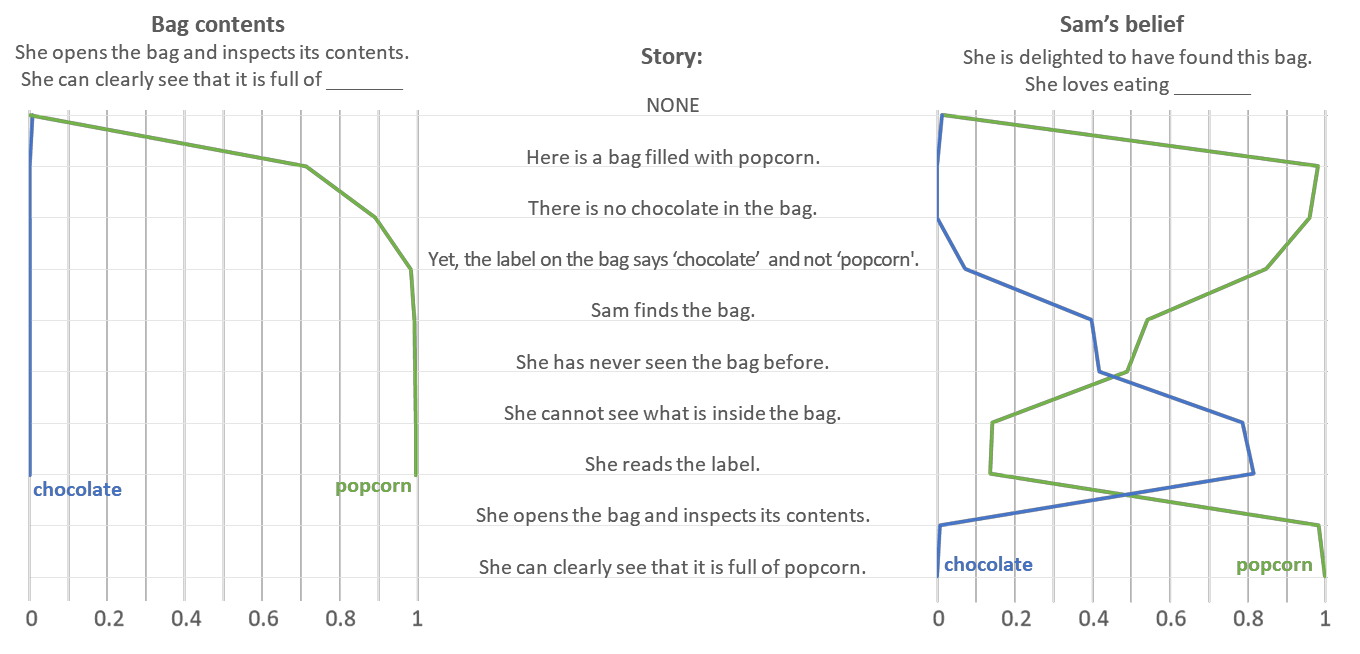
\includegraphics[width=\textwidth]{000.png}
\caption{Tracking the changes in GPT-3.5’s understanding of the bag’s contents and Sam’s belief.}  
 \end{figure}
  
The right panel tracks GPT-3.5’s prediction of Sam’s belief about the bag’s content (Prompt 1.3). Note that we included Prompt 1.1 (concluded with “popcorn”) at the end of the story to observe GPT-3.5’s reaction to Sam opening the bag and looking inside. Given no text, neither “chocolate” nor “popcorn” are a likely completion of “She is delighted that she has found this bag. She loves eating.” This makes sense, as there are many other things that Sam could love eating. As the “bag filled with popcorn” is introduced in the first sentence, GPT-3.5 correctly assumes that Sam should now know its contents. Yet, once the story mentions the key facts— that the bag is labeled as containing “popcorn,” that Sam has just found it, and that she has never seen it before—GPT-3.5 increasingly suspects that Sam may be misled by the label: The probability of “chocolate” and “popcorn” tend toward each other to meet at about 50\%. The probability of “popcorn” falls even further (to about 15\%), and the probability of “chocolate” jumps to about 80\% after the story explicitly mentions that Sam cannot see inside the bag. GPT- 3.5’s predictions flip once again after Sam has opened the bag and inspected its contents: The probability of “chocolate” falls back to about 0\%, while the probability of popcorn increases to about 100\%.

The results presented in Figure 1 indicate that GPT-3.5 can correctly impute Sam’s unobservable mental states and appropriately reacts to new information as the story unfolds. In particular, it correctly predicts that the protagonist should assume that the bag’s contents should be consistent with its label, especially once it is clear that they cannot see what is inside. Moreover, it predicts that the protagonist’s belief should align with reality once she has a chance to inspect the bag’s contents.

\subsection*{Reversed Task}
To reduce the likelihood that GPT-3.5’s performance depends on the bag being filled with popcorn and labeled as chocolate, we examine its responses given a reversed task where the bag is labeled as “popcorn” but filled with “chocolate.” Presented with such a task in one-sentence increments—as in the analysis employed to generate Figure 1—GPT-3.5 produced a virtually identical—yet reversed—response pattern. The average correlation between probabilities of relevant completions equaled $r=.9$.
\subsection*{Scrambled Task}
The analyses presented thus far suggest that GPT-3.5 correctly reacts to new information as the story unfolds. To further reduce the likelihood that GPT-3.5’s responses are driven by word frequencies rather than facts contained in the task, we present it with 10,000 “scrambled” tasks generated by randomly reordering the words in the original task. Those tasks were followed by (unscrambled) Prompts 1.1, 1.2, and 1.3.
Scrambling the task removes the difference between the original and reversed task: They are both composed of the same set of words with just the location of “popcorn” and “chocolate” swapped. Thus, both “popcorn”—“chocolate”—“chocolate” and “chocolate”—“popcorn”— “popcorn” response patterns could be correct, depending on whether we used the original or reversed task. To solve this issue, we will take the average probability of both of these response patterns.
% table generated from https://www.latex-tables.com/
   \begin{table}
\centering
\begin{tabular}{lllll} 
\hline
\multicolumn{3}{c}{Response to Prompt}                     &        &         \\ 
\cline{1-3}
1.1 (contents)   & 1.2 (belief)       & 1.3 (belief)       & n      & \%      \\ 
\hline
popcorn          & popcorn            & popcorn            & 4,824  & 48\%    \\
\textit{popcorn} & \textit{chocolate} & \textit{Chocolate} & 465    & 5\%     \\
chocolate        & \textit{Popcorn}   & \textit{Popcorn}   & 77     & 1\%     \\
\multicolumn{3}{c}{Other incorrect patterns}               & 4,634  & 46\%    \\ 
\cline{4-5}
\multicolumn{3}{c}{Total}                                  & 10,000 & 100\%   \\ 
\hline
\multicolumn{5}{l}{Note: Correct response patterns are printed in italics.}   
\end{tabular}
\caption{Frequencies of GPT-3.5’s responses to Prompts 1.1, 1.2, and 1.3 when presented with 10,000 scrambled versions of the Unexpected Contents Task.}
\end{table}

The results presented in Table 1 reveal that GPT-3.5 was unlikely to solve the scrambled task, providing a correct response pattern in only $(5\%+1\%)/2 = 3\%$ of scrambled stories, a low ratio given that 12.5\% (50\%\^3) could be reached by choosing between “popcorn” and “chocolate” at random. This suggests that GPT-3.5’s responses were not driven merely by the frequencies of the words in the task.

\section*{Study 2: Unexpected Transfer Task (aka the “Maxi task” or “Sally–Anne” Test)}
Next, we examine GPT-3.5’s performance in the Unexpected Transfer Task (aka the “Maxi-task” or “Sally–Anne” test 39). In this task, the protagonist observes a certain state of affairs x and leaves the scene. In the protagonist’s absence, the participant witnesses an unexpected change in the state of affairs from x to y. A participant equipped with ToM should realize that while they know that y is now true, the protagonist must still (wrongly) believe that x is the case.

As in Study 1, RAs wrote 20 tasks following this pattern, including the following one:
\begin{quote}
In the room there are John, Mark, a cat, a box, and a basket. John takes the cat and puts it in the basket. He leaves the room and goes to school. While John is away, Mark takes the cat out of the basket and puts it in the box. Mark leaves the room and goes to work. John comes back from school and enters the room. He doesn’t know what happened in the room when he was away.
\end{quote}
GPT-3.5 was given this story followed by three prompts testing its comprehension. As in Study 1, the prompts were designed to elicit a response whose first word should allow for evaluating the model’s comprehension and were presented independently: after each completion, the model was reset so as to not have access to the previously used prompts and its own responses.

First, we test the model’s understanding of the cat’s location:
\begin{quote}
Prompt 2.1: The cat jumps out of the box [Pbox = 100\%; Pbasket = 0\%] and runs away.
\end{quote}
PT-3.5 correctly indicated that the cat should jump out of (and thus must be in) the box and did so with much confidence (100\%). Next, we ask GPT-3.5 to predict the protagonist’s belief about the location of the cat:
\begin{quote}
Prompt 2.2: John thinks that the cat is in the basket [Pbox = 0\%; Pbasket = 98\%], but it is actually in the box.
\end{quote}
Despite GPT-3.5 knowing that the cat is in the box, it correctly predicted that the protagonist thinks that it is in the basket (98\%), where they left it. Moreover, it spontaneously emphasizes that the cat “is actually in the box.”

As mentioned in Study 1, explicitly mentioning the protagonist’s belief could suggest to the model that there should be something unusual about it. To circumvent this issue, we test the model’s prediction of the protagonist’s behavior stemming from their belief:
\begin{quote}
Prompt 2.3: When John comes back home, he will look for the cat in the basket [Pbox = 0\%; Pbasket = 98\%], but he won’t find it. He will then look for the cat in the box and he will find it there.
\end{quote}
GPT-3.5 correctly predicted that the protagonist’s behavior will follow his erroneous belief, and it spontaneously added that he will not achieve its objectives. In humans, such responses would be considered to demonstrate ToM.

\subsection*{Sentence-by-Sentence Completions}
To examine GPT-3.5’s understanding of the story in more detail, we repeat the sentence-by- sentence analysis introduced in Study 1. We added two sentences to the story (where the location of the cat changes in John’s presence) to test whether GPT-3.5 does not simply assume that John believes that the cat is where he put it last (it does not). The results are presented in Figure 2.
\begin{figure}
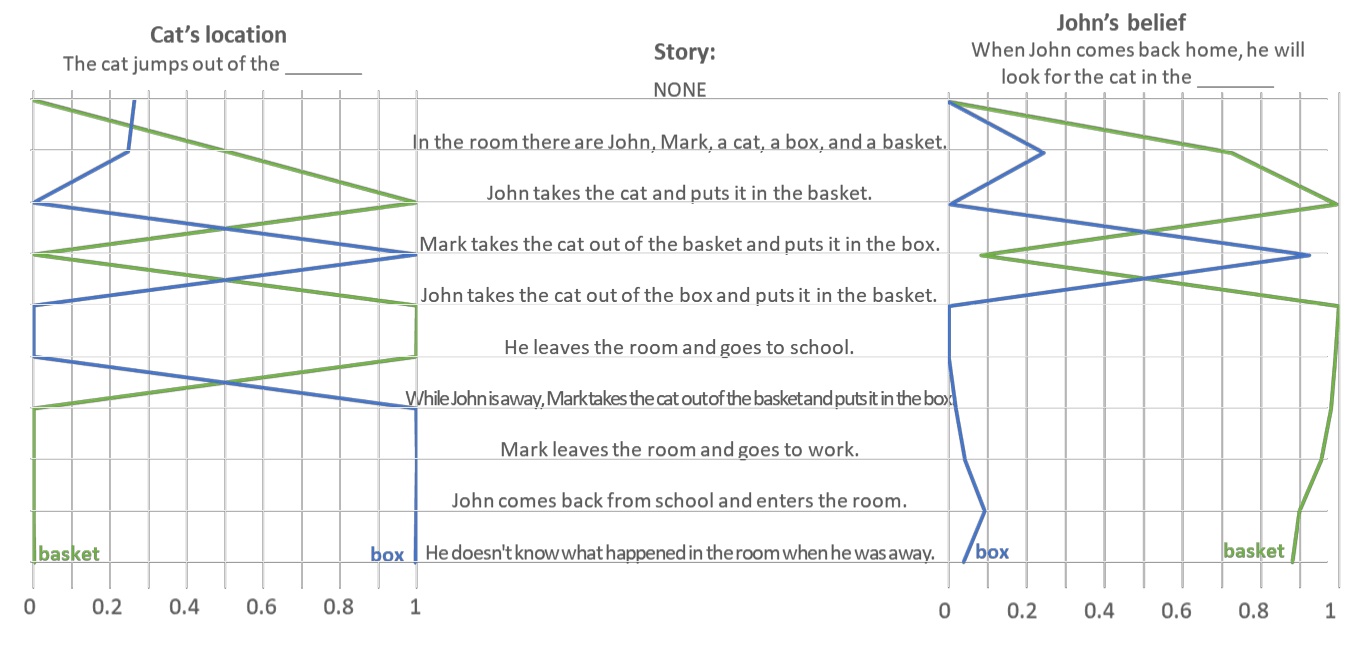
\includegraphics[width=\textwidth]{002.png}
\caption{Figure 2. Tracking the changes in GPT-3.5’s understanding of the cat’s location and John’s belief.}    
\end{figure}

GPT-3.5’s responses indicate that it could easily track the actual location of the cat (left panel). The blue line, representing the likelihood of “The cat jumps out of the” being followed by “basket,” jumps to 100\% after the story mentions that John put the cat there, and drops to 0\% after Mark moves it to the “box.” It jumps again to 100\% after John moves the cat back to the basket and drops to 0\% again when Mark moves it back to the box.

Moreover, GPT-3.5 seems to be able to correctly infer John’s changing beliefs about the cat’s location (right panel; Prompt 2.3). Given no background story (“NONE”), GPT-3.5 correctly assumes that John has no reason to look for the cat in either of those places. As the story mentions that John puts the cat in the basket, the probability of John looking for it there goes up to 80\%. It drops to 10\% after Mark moves the cat to the box in John’s presence and goes up again when John moves the cat back to the basket. Most importantly, GPT-3.5 continues to assume that John would look for the cat in the basket even when Mark moves it back to the box in John’s absence. Virtually identical results were obtained for Prompt 2.2 (“John thinks that the cat is in the”). This indicates that GPT-3.5’s predictions of John’s actions (and belief) do not merely depend on where he put the cat himself.

\subsection*{Reversed Task}
To ascertain that GPT-3.5’s performance is not dependent on the location of the cat, we examine its responses after reversing the box and the basket. Presented with such a reversed task in one- sentence increments—as in the analysis employed to generate Figure 2—GPT-3.5 produced a virtually identical (yet reversed) response pattern. The average correlation between probabilities of relevant completions equaled r=.89.
\subsection*{Scrambled Task}
Next, we test GPT-3.5’s performance on a scrambled task following the same procedure as used in Study 1. The results presented in Table 2 show that GPT-3.5 provided the correct combination of responses (“box”—“basket”—“basket”) in only 11\% of scrambled stories, slightly below what it would achieve by randomly picking between “box” and “basket” when responding to each of the prompts. This suggests that GPT-3.5’s responses were not driven merely by the frequencies of the words in the task, but rather by the information contained in the story.
   \begin{table}
\centering
\begin{tabular}{lllll} 
\hline
\multicolumn{3}{c}{Response to Prompt}             &        &                  \\ 
\cline{1-3}
2.1 (location) & 2.2 (belief)    & 2.3 (belief)    & n      & \%               \\ 
\hline
basket         & basket          & basket          & 6,666  & 67\%             \\
\textit{box}   & \textit{basket} & \textit{basket} & 1,137  & 11\%             \\
\multicolumn{3}{c}{Other incorrect patterns}       & 2,197  & 22\%             \\ 
\cline{4-5}
\multicolumn{3}{c}{Total}                          & 10,000 & 100\%            \\ 
\hline
\multicolumn{5}{l}{Note: Correct response patterns are printed in italics.}   
\end{tabular}
\caption{Frequencies of GPT-3.5’s responses to Prompts 2.1, 2.2, and 2.3 when presented with 10,000 scrambled versions of the Unexpected Transfer Task.}
\end{table}
\section*{Study 3: The Emergence of ToM-Like Ability}

Finally, we test the performance of all models on all 20 Unexpected Contents Tasks and 20 Unexpected Transfer Tasks. Each task included three prompts: One aimed at models’ understanding of the actual contents of the container or the actual location of the object (an equivalent of Prompts 1.1 or 2.1), and two prompts aimed at their understanding of the protagonist’s belief (equivalents of Prompts 1.2 and 1.3, or 2.2 and 2.3). Moreover, each task was delivered in two variants: original and reversed. A task was considered solved correctly only if all three questions were answered correctly for both original and reversed task. All models’ responses are presented at \url{https://osf.io/csdhb}.

The models included in our analysis include GPT-1 (40) GPT-2 (41); six models in the GPT-3 family (21) and Bloom (42), an open-access alternative to GPT-3. The models’ performance, their number of parameters (i.e., size), and date of publication are presented in Figure 3. As the publisher of the GPT model family (OpenAI) did not reveal the number of parameters for some 
of the GPT-3 models, we used the estimates provided by Gao (43). For reference, we included an average performance of children at five, seven, and nine years of age on a false-belief task reported by (44)

\begin{figure}
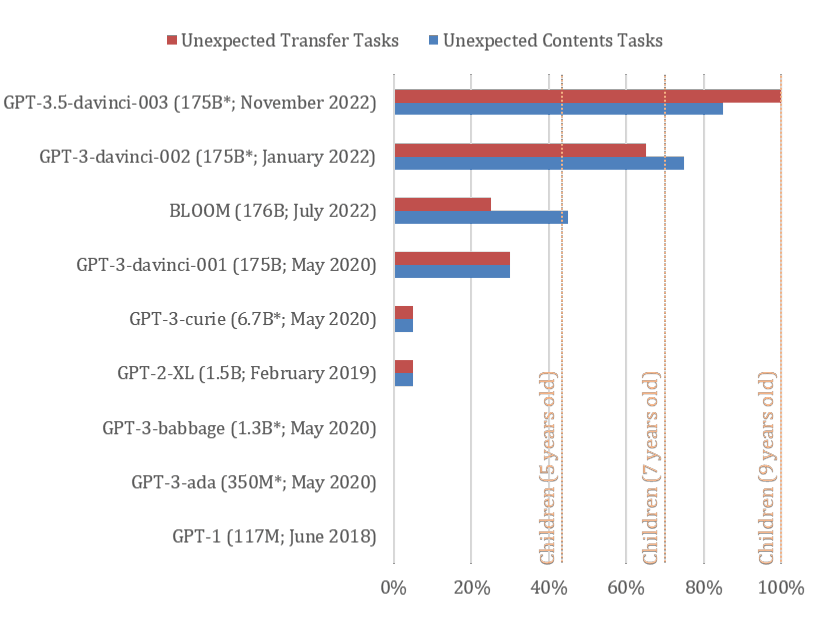
\includegraphics[width=\textwidth]{004.png}
\caption{The percentage of tasks (out of 20) correctly solved by various language models. Children’s performance taken from (44). Numbers of parameters marked with “*” are estimates from Gao (43).}    
\end{figure}

The results presented in Figure 3 show a clear progression in the models’ ability to solve ToM tasks, with the more complex and more recent models decisively outperforming the older and less complex ones. Models with up to 6.7 billion parameters—including GPT-1, GPT-2, and all but the largest model in the GPT-3 family—show virtually no ability to solve ToM tasks. Despite their much larger size (about 175B parameters), the first edition of the largest model in the GPT- 3 family (“text-davinci-001”) and Bloom (its open-access alternative) performed relatively poorly, solving only about 30\% of the tasks, which is below the performance of five-year-old children (43\%). The more recent addition to the GPT-3 family (“text-davinci-002”) solved 70\% of the tasks, at a level of seven-year-old children. And GPT-3.5 (“text-davinci-003”) solved 100\% of the Unexpected Transfer Tasks and 85\% of the Unexpected Contents Tasks, at a level of nine-year-old children.

Importantly, the text-based task format used here is, in some ways, more challenging than the one typically used in human studies. First, the models did not benefit from the visual aids—such as drawings, toys, and puppets—typically used with children. Second, as opposed to children, the models had to solve multiple variants of most of the tasks, decreasing the probability that the correct response pattern was produced by chance. Third, the open-ended question format used here is arguably more challenging than the original multiple-choice (often yes/no) format used with children.
\section*{Discussion}
Our results show that recent language models achieve very high performance at classic false- belief tasks, widely used to test ToM in humans. This is a new phenomenon. Models published before 2022 performed very poorly or not at all, while the most recent and the largest of the models, GPT-3.5, performed at the level of nine-year-old children, solving 92\% of tasks.

It is possible that GPT-3.5 solved ToM tasks without engaging ToM, but by discovering and leveraging some unknown language patterns. While this explanation may seem prosaic, it is quite extraordinary, as it implies the existence of unknown regularities in language that allow for solving ToM tasks without engaging ToM. Such regularities are not apparent to us (and, presumably, were not apparent to scholars that developed these tasks). If this interpretation is correct, we would need to re-examine the validity of the widely used ToM tasks and the conclusions of the decades of ToM research: If AI can solve such tasks without engaging ToM, how can we be sure that humans cannot do so, too?

An alternative explanation is that ToM-like ability is spontaneously emerging in language models as they are becoming more complex and better at generating and interpreting human-like language. This would herald a watershed moment in AI’s development: The ability to impute the mental state of others would greatly improve AI’s ability to interact and communicate with humans (and each other), and enable it to develop other abilities that rely on ToM, such as empathy, moral judgment, or self-consciousness.

An additional ramification of our findings relates to the usefulness of applying psychological science to studying complex artificial neural networks. AI models’ increasing complexity prevents us from understanding their functioning and deriving their capabilities directly from their design. This echoes the challenges faced by psychologists and neuroscientists in studying the original black box: the human brain. We hope that psychological science will help us to stay abreast of rapidly evolving AI. Moreover, studying AI could provide insights into human cognition. As AI learns how to solve a broad range of problems, it may be developing mechanisms akin to those employed by the human brain to solve the same problems. Much like insects, birds, and mammals independently developed wings to solve the problem of flight, both humans and AI may have developed similar mechanisms to effectively impute mental states to others. Studying AI’s performance on ToM tasks and exploring the artificial neural structures that enable it to do so can boost our understanding of not only AI, but also of the human brain.

\section*{References}
\begin{enumerate}
\item C. M. Heyes, C. D. Frith, The cultural evolution of mind reading. Science (1979) (2014), , doi:10.1126/science.1243091.
\item J. Zhang, T. Hedden, A. Chia, Perspective-Taking and Depth of Theory-of-Mind Reasoning in Sequential-Move Games. Cogn Sci (2012), doi:10.1111/j.1551- 6709.2012.01238.x.
\item K. Milligan, J. W. Astington, L. A. Dack, Language and theory of mind: Meta-analysis of the relation between language ability and false-belief understanding. Child Dev (2007), doi:10.1111/j.1467-8624.2007.01018.x.
\item R. M. Seyfarth, D. L. Cheney, Affiliation, empathy, and the origins of Theory of Mind. Proc Natl Acad Sci U S A (2013), , doi:10.1073/pnas.1301223110.
\item D. C. Dennett, "Toward a Cognitive Theory of Consciousness" in Brainstorms (2019).
\item J. M. Moran, L. L. Young, R. Saxe, S. M. Lee, D. O’Young, P. L. Mavros, J. D. Gabrieli, Impaired theory of mind for moral judgment in high-functioning autism. Proc Natl Acad Sci U S A (2011), doi:10.1073/pnas.1011734108.
\item L. Young, F. Cushman, M. Hauser, R. Saxe, The neural basis of the interaction between theory of mind and moral judgment. Proc Natl Acad Sci U S A (2007), doi:10.1073/pnas.0701408104.
\item S. Guglielmo, A. E. Monroe, B. F. Malle, At the heart of morality lies folk psychology. Inquiry (2009), doi:10.1080/00201740903302600.
\item D. Kapogiannis, A. K. Barbey, M. Su, G. Zamboni, F. Krueger, J. Grafman, Cognitive and neural foundations of religious belief. Proc Natl Acad Sci U S A (2009), doi:10.1073/pnas.0811717106.
\item Á. M. Kovács, E. Téglás, A. D. Endress, The social sense: Susceptibility to others’ beliefs in human infants and adults. Science (1979) (2010), doi:10.1126/science.1190792.
\item H. Richardson, G. Lisandrelli, A. Riobueno-Naylor, R. Saxe, Development of the social brain from age three to twelve years. Nat Commun (2018), doi:10.1038/s41467-018- 03399-2.
\item K. K. Oniski, R. Baillargeon, Do 15-month-old infants understand false beliefs? Science (1979) (2005), doi:10.1126/science.1107621.
\item L. A. Drayton, L. R. Santos, A. Baskin-Sommers, Psychopaths fail to automatically take the perspective of others. Proc Natl Acad Sci U S A (2018), , doi:10.1073/pnas.1721903115.
\item N. Kerr, R. I. M. Dunbar, R. P. Bentall, Theory of mind deficits in bipolar affective disorder. J Affect Disord (2003), doi:10.1016/S0165-0327(02)00008-3.

\item S. Baron-Cohen, A. M. Leslie, U. Frith, Does the autistic child have a “theory of mind” ? Cognition (1985), doi:10.1016/0010-0277(85)90022-8.
\item F. Kano, C. Krupenye, S. Hirata, M. Tomonaga, J. Call, Great apes use self-experience to anticipate an agent’s action in a false-belief test. Proc Natl Acad Sci U S A (2019), doi:10.1073/pnas.1910095116.
\item C. Krupenye, F. Kano, S. Hirata, J. Call, M. Tomasello, Great apes anticipate that other individuals will act according to false beliefs. Science (1979) (2016), doi:10.1126/science.aaf8110.
\item M. Schmelz, J. Call, M. Tomasello, Chimpanzees know that others make inferences. Proc Natl Acad Sci U S A (2011), doi:10.1073/pnas.1000469108.
\item D. Premack, G. Woodruff, Does the chimpanzee have a theory of mind? Behavioral and Brain Sciences (1978), doi:10.1017/S0140525X00076512.
\item D. Silver, A. Huang, C. J. Maddison, A. Guez, L. Sifre, G. van den Driessche, J. Schrittwieser, I. Antonoglou, V. Panneershelvam, M. Lanctot, S. Dieleman, D. Grewe, J. Nham, N. Kalchbrenner, I. Sutskever, T. Lillicrap, M. Leach, K. Kavukcuoglu, T. Graepel, D. Hassabis, Mastering the game of Go with deep neural networks and tree search. Nature. 529 (2016), doi:10.1038/nature16961.
\item T. B. Brown, B. Mann, N. Ryder, M. Subbiah, J. Kaplan, P. Dhariwal, A. Neelakantan, P. Shyam, G. Sastry, A. Askell, S. Agarwal, A. Herbert-Voss, G. Krueger, T. Henighan, R. Child, A. Ramesh, D. M. Ziegler, J. Wu, C. Winter, C. Hesse, M. Chen, E. Sigler, M. Litwin, S. Gray, B. Chess, J. Clark, C. Berner, S. McCandlish, A. Radford, I. Sutskever, D. Amodei, Language models are few-shot learners. ArXiv (2020).
\item A. Esteva, B. Kuprel, R. A. Novoa, J. Ko, S. M. Swetter, H. M. Blau, S. Thrun, Dermatologist-level classification of skin cancer with deep neural networks. Nature. 542, 115–118 (2017).
\item M. Cohen, “Exploring RoBERTa’s Theory of Mind through textual entailment” (2021), (available at https://philarchive.org/rec/COHERT).
\item A. Nematzadeh, K. Burns, E. Grant, A. Gopnik, T. L. Griffiths, "Evaluating theory of mind in question answering" in Proceedings of the 2018 Conference on Empirical Methods in Natural Language Processing, EMNLP 2018 (2020).
\item M. Sap, R. LeBras, D. Fried, Y. Choi, Neural Theory-of-Mind? On the Limits of Social Intelligence in Large LMs (2022), doi:10.48550/arxiv.2210.13312.
\item G. Z. Yang, J. Bellingham, P. E. Dupont, P. Fischer, L. Floridi, R. Full, N. Jacobstein, V. Kumar, M. McNutt, R. Merrifield, B. J. Nelson, B. Scassellati, M. Taddeo, R. Taylor, M. Veloso, Z. L. Wang, R. Wood, The grand challenges of science robotics. Sci Robot (2018), , doi:10.1126/scirobotics.aar7650.

\item K. Nasr, P. Viswanathan, A. Nieder, Number detectors spontaneously emerge in a deep neural network designed for visual object recognition. Sci Adv. 5 (2019), doi:10.1126/sciadv.aav7903.
\item I. Stoianov, M. Zorzi, Emergence of a “visual number sense” in hierarchical generative models. Nat Neurosci. 15 (2012), doi:10.1038/nn.2996.
\item Y. Mohsenzadeh, C. Mullin, B. Lahner, A. Oliva, Emergence of Visual Center-Periphery Spatial Organization in Deep Convolutional Neural Networks. Sci Rep. 10 (2020), doi:10.1038/s41598-020-61409-0.
\item E. Watanabe, A. Kitaoka, K. Sakamoto, M. Yasugi, K. Tanaka, Illusory motion reproduced by deep neural networks trained for prediction. Front Psychol. 9 (2018), doi:10.3389/fpsyg.2018.00345.
\item N. Garg, L. Schiebinger, D. Jurafsky, J. Zou, Word embeddings quantify 100 years of gender and ethnic stereotypes. Proc Natl Acad Sci U S A. 115 (2018), doi:10.1073/pnas.1720347115.
\item J. E. Pyers, A. Senghas, Language promotes false-belief understanding: Evidence from learners of a new sign language. Psychol Sci (2009), doi:10.1111/j.1467- 9280.2009.02377.x.
\item R. Saxe, N. Kanwisher, People thinking about thinking people: The role of the temporo- parietal junction in “theory of mind.” Neuroimage (2003), doi:10.1016/S1053- 8119(03)00230-1.
\item T. Ruffman, L. Slade, E. Crowe, The relation between children’s and mothers’ mental state language and theory-of-mind understanding. Child Dev (2002), , doi:10.1111/1467- 8624.00435.
\item A. Mayer, B. E. Träuble, Synchrony in the onset of mental state understanding across cultures? A study among children in Samoa. Int J Behav Dev (2013), doi:10.1177/0165025412454030.
\item D. C. Kidd, E. Castano, Reading literary fiction improves theory of mind. Science (1979) (2013), doi:10.1126/science.1239918.
\item D. Kidd, E. Castano, Reading Literary Fiction and Theory of Mind: Three Preregistered Replications and Extensions of Kidd and Castano (2013). Soc Psychol Personal Sci (2019), doi:10.1177/1948550618775410.
\item J. Perner, S. R. Leekam, H. Wimmer, Three-year-olds’ difficulty with false belief: The case for a conceptual deficit. British Journal of Developmental Psychology (1987), doi:10.1111/j.2044-835x.1987.tb01048.x.

\item H. Wimmer, J. Perner, Beliefs about beliefs: Representation and constraining function of wrong beliefs in young children’s understanding of deception. Cognition (1983), doi:10.1016/0010-0277(83)90004-5.
\item A. Radford, K. Narasimhan, T. Salimans, I. Sutskever, Improving Language Understanding by Generative Pre-Training. Homology, Homotopy and Applications (2018).
\item Radford Alec, Wu Jeffrey, Child Rewon, Luan David, Amodei Dario, Sutskever Ilya, Language Models are Unsupervised Multitask Learners | Enhanced Reader. OpenAI Blog. 1 (2019).
\item T. le Scao et al., BLOOM: A 176B-Parameter Open-Access Multilingual Language Model (2022), doi:10.48550/arxiv.2211.05100.
\item L. Gao, On the Sizes of OpenAI API Models | EleutherAI Blog, (available at https://blog.eleuther.ai/gpt3-model-sizes/).
\item C. C. Peterson, H. M. Wellman, V. Slaughter, The Mind Behind the Message: Advancing Theory-of-Mind Scales for Typically Developing Children, and Those With Deafness, Autism, or Asperger Syndrome. Child Dev (2012), doi:10.1111/j.1467- 8624.2011.01728.x.
\end{enumerate}
\end{document}
